% ---------------------------------------------------------------- 10 Input/output
\begin{frame}{Input and output representation}
  \centering
  \begin{tikzpicture}
    \draw[soft,dashed,thin,fill=accent!4] (0,0.3) rectangle (1.45,1.8);
    \draw[soft,thin,fill=black!2] (0.16,0.46) rectangle (1.29,1.64);
    \node[font=\scriptsize,align=center,anchor=north] at (0.72,0.18) {symmetric padding\\mirrored edges};
    \draw[flow] (1.55,1.05) -- (2.0,1.05);
    \draw[soft,dashed,thin,fill=accent!4] (2.1,0.3) rectangle (3.55,1.8);
    \draw[soft,thin,fill=black!2] (2.26,0.46) rectangle (3.39,1.64);
    \draw[accent,dashed,thin] (2.13,0.33) rectangle ++(0.7,0.7);
    \draw[accent!45,dashed,thin] (2.48,0.68) rectangle ++(0.7,0.7);
    \node[font=\scriptsize,align=center,anchor=north] at (2.82,0.18) {$64{\times}64$ patches\\stride 32};
    \draw[flow] (3.65,1.05) -- (4.15,1.05);
    \draw[soft,thin,fill=white] (4.3,0.5) rectangle ++(1.0,1.0);
    \draw[black!8,step=0.2,shift={(4.3,0.5)}] (0,0) grid (1.0,1.0);
    \draw[accent!70,thick] (4.3,0.5) rectangle ++(1.0,1.0);
    \node[font=\scriptsize,anchor=south] at (4.8,1.85) {primary $|A|$};
    \foreach \i in {3,2,1} \draw[soft,thin,fill=black!2] (5.6+0.07*\i,0.5+0.07*\i) rectangle ++(1.0,1.0);
    \draw[soft,thin,fill=white] (5.6,0.5) rectangle ++(1.0,1.0);
    \draw[black!8,step=0.2,shift={(5.6,0.5)}] (0,0) grid (1.0,1.0);
    \node[font=\scriptsize,anchor=south] at (6.2,1.85) {4 secondary $|A|$};
    \foreach \i in {3,2,1} \draw[soft,thin,fill=black!2] (7.2+0.07*\i,0.5+0.07*\i) rectangle ++(1.0,1.0);
    \draw[soft,thin,fill=white] (7.2,0.5) rectangle ++(1.0,1.0);
    \begin{scope} \clip (7.2,0.5) rectangle ++(1.0,1.0); \foreach \r in {0.45,0.62,...,1.85} \draw[accent!30,thin] (8.55,0.2) circle (\r); \end{scope}
    \node[font=\scriptsize,anchor=south] at (7.8,1.85) {4 IFG phases};
    \draw[decorate,decoration={brace,amplitude=4pt,mirror},soft] (4.3,0.35) -- (8.41,0.35);
    \node[font=\scriptsize,text=soft,anchor=north] at (6.36,0.12) {9 input channels};
    \draw[flow] (8.65,1.05) -- (9.1,1.05);
    \foreach \x/\h in {9.25/1.5,9.6/1.1,9.95/1.1,10.3/1.5} \draw[accent!70,thick,fill=accent!6,rounded corners=1pt] (\x,1.05-\h/2) rectangle ++(0.22,\h);
    \node[font=\scriptsize,anchor=north] at (9.89,0.2) {$f_\theta$};
    \draw[flow] (10.65,1.05) -- (11.05,1.05);
    \foreach \x/\lbl in {11.2/{$a_1$},11.61/{$\mu_1$},12.02/{$\sigma_1$},12.5/{$a_2$},12.91/{$\mu_2$},13.32/{$\sigma_2$}} { \draw[soft,thin,fill=white] (\x,0.86) rectangle ++(0.38,0.38); \node[font=\tiny,anchor=north] at (\x+0.19,0.78) {\lbl}; }
    \draw[decorate,decoration={brace,amplitude=4pt},soft] (11.2,1.36) -- (13.7,1.36);
    \node[font=\scriptsize,text=soft,anchor=south] at (12.45,1.57) {$3K$ maps, interleaved};
  \end{tikzpicture}
  \\[10pt]
  \small
  \begin{itemize}
    \item Scenes are symmetrically padded (edge-mirrored) so the $64\times 64$, stride-32
          patch grid tiles them exactly; sliding-window stitching undoes the overlap at inference.
    \item The $3K$ output channels are interleaved per scatterer ---
          $a_1,\mu_1,\sigma_1,a_2,\mu_2,\sigma_2,\dots$ --- not grouped by parameter type.
    \item Outputs live in normalized space; denormalised and clamped to physical bounds
          before any curve is reconstructed.
    \item Current configuration $K{=}2$ (6 maps); the $K{=}5$ variant (15 maps) in development.
  \end{itemize}
\end{frame}

% ---------------------------------------------------------------- 10b Real channel distributions
\begin{frame}{Two input channels, two regimes}
  \begin{columns}[T]
    \begin{column}{0.5\textwidth}
      \centering
      {\small\textbf{\textcolor{accent}{primary amplitude}}}\\[3pt]
      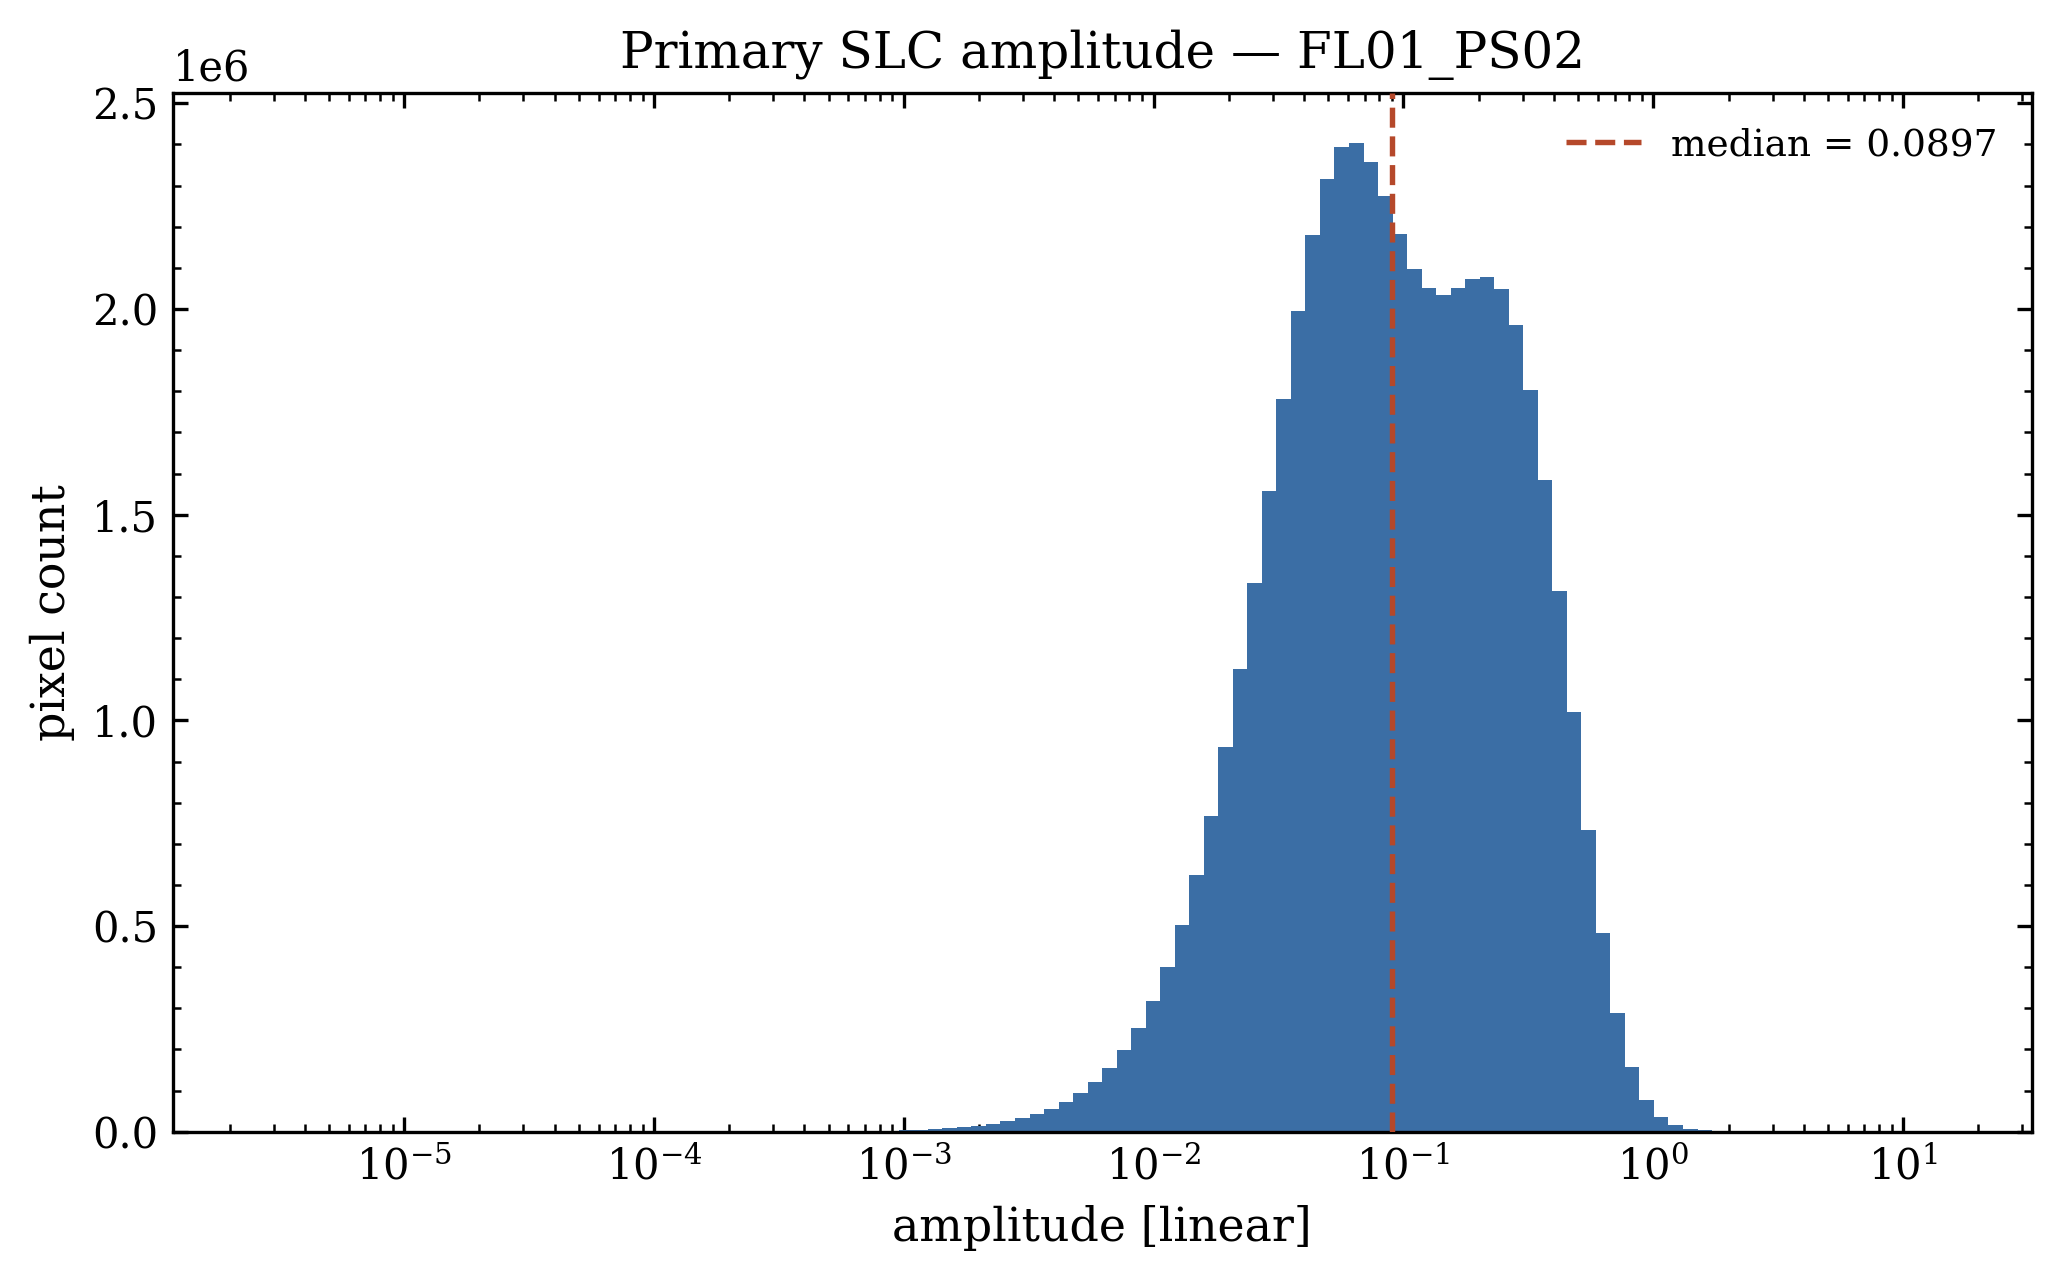
\includegraphics[width=\linewidth]{../figures/preprocessing_inference/channel_distributions/pass_00_FL01_PS02_amplitude.png}\\[3pt]
      {\scriptsize\color{soft} Log-scaled axis: the bulk sits near $10^{-1}$ but the tail runs past $10^{0}$ --- orders of magnitude in one channel. \textcolor{accent}{Heavy-tailed} $\rightarrow$ robust log1p scaling.}
    \end{column}
    \begin{column}{0.5\textwidth}
      \centering
      {\small\textbf{\textcolor{good}{interferogram phase}}}\\[3pt]
      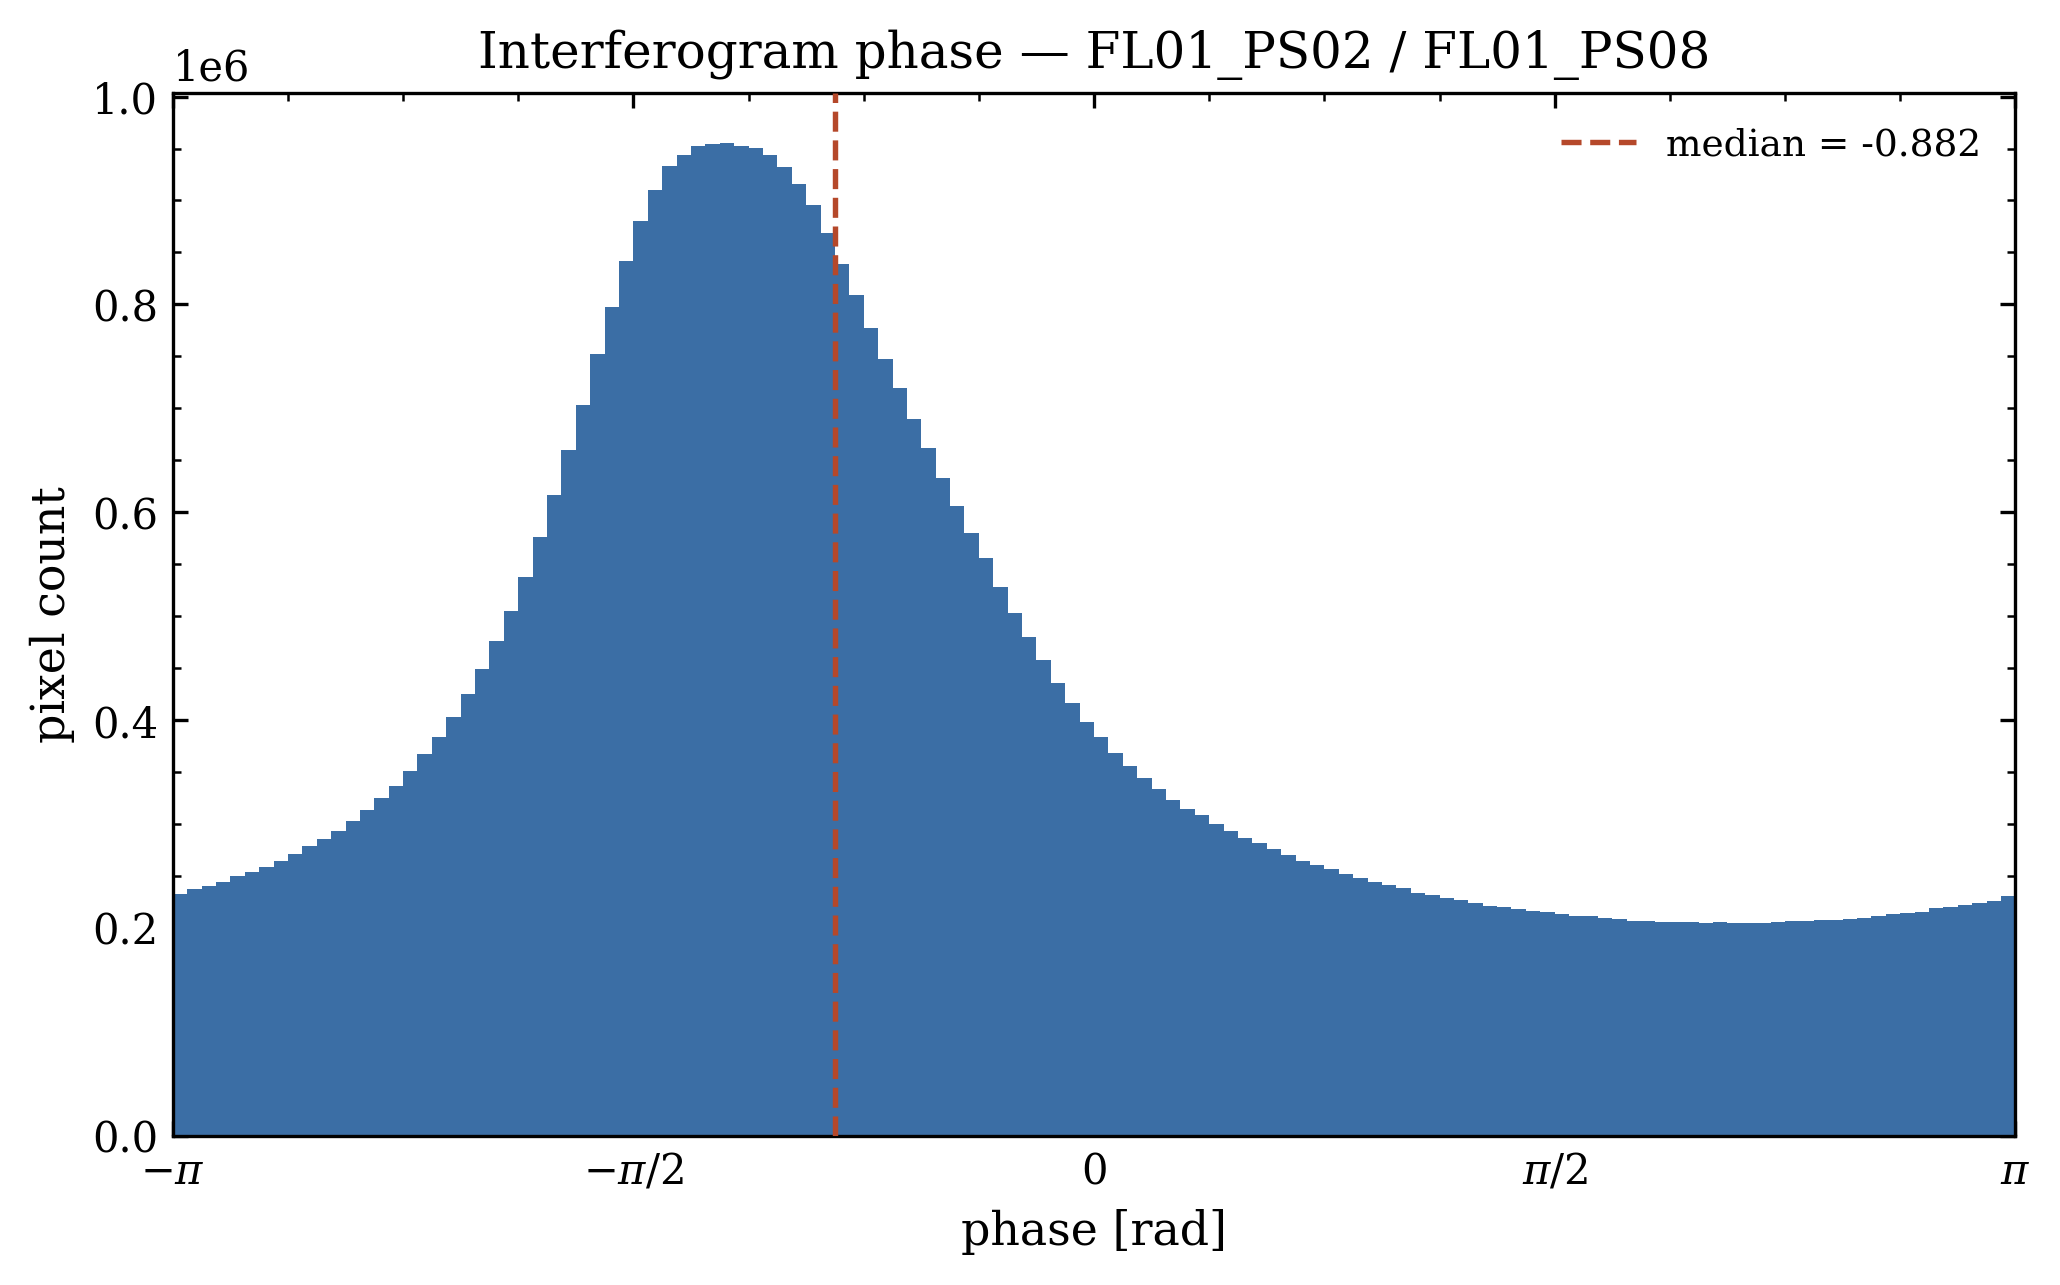
\includegraphics[width=\linewidth]{../figures/preprocessing_inference/channel_distributions/interferogram_03_FL01_PS08_phase.png}\\[3pt]
      {\scriptsize\color{soft} Confined to $[-\pi,\pi]$ by construction, a single broad mode --- no tail to tame. \textcolor{good}{Bounded by physics} $\rightarrow$ fixed $\div\,\pi$.}
    \end{column}
  \end{columns}
  \vspace{5pt}
  \centering
  {\footnotesize Real F-SAR channels (primary PS02, IFG PS02/PS08). The nine inputs split cleanly into these two shapes --- and the normalization strategy (next) follows the split.}
\end{frame}

% ---------------------------------------------------------------- 12 Strategy table
\begin{frame}{Per-channel normalization --- old $\to$ new, channel by channel}
  \begin{columns}[c]
    \begin{column}{0.58\textwidth}
      \centering
      \scriptsize
      \renewcommand{\arraystretch}{1.75}
      \setlength{\tabcolsep}{3pt}
      {\color{soft} z-score --- standard score \quad$\cdot$\quad IQR --- interquartile range}\\[5pt]
      \begin{tabular}{@{}l l c l l@{}}
        \toprule
        channel & old & & new & why \\
        \midrule
        pass / mag     & \textcolor{soft}{z-score (log1p)}        & $\to$ & \textbf{\textcolor{accent}{robust IQR (log1p)}} & tail sets $\mu$, $\sigma$ \\
        ifg / phase    & \textcolor{soft}{min--max ($p_{99.9}$)}  & $\to$ & \textbf{\textcolor{good}{fixed $\div\,\pi$}}    & bounded by physics \\
        \addlinespace
        out / $a$      & \textcolor{soft}{z-score}                & $\to$ & \textbf{\textcolor{accent}{robust IQR (log1p)}} & heavy-tailed target \\
        out / $\sigma$ & \textcolor{soft}{z-score}                & $\to$ & \textbf{\textcolor{accent}{robust IQR (log1p)}} & heavy-tailed target \\
        out / $\mu$    & \textcolor{soft}{z-score}                & $=$   & \textcolor{soft}{z-score \emph{(kept)}}         & bounded to sampling range \\
        \bottomrule
      \end{tabular}
      \\[19pt]
      \begin{minipage}[c]{0.36\linewidth}
        \centering
        \mbox{\small\color{soft} $\tilde x = \dfrac{x - \mu}{\sigma}$}
      \end{minipage}\hfill
      \begin{minipage}[c]{0.60\linewidth}
        \scriptsize\color{soft}
        \textbf{old --- moments fit the tail.} Rare bright pixels drag $\mu$ and inflate $\sigma$; the bulk compresses into a narrow band.\par
      \end{minipage}
      \\[9pt]
      \begin{minipage}[c]{0.36\linewidth}
        \centering
        \mbox{\small\color{accent} $\tilde x = \dfrac{\log(1{+}x) - \mathrm{med}}{Q_3 - Q_1}$}
      \end{minipage}\hfill
      \begin{minipage}[c]{0.60\linewidth}
        \scriptsize\color{ink}
        \textbf{\textcolor{accent}{new --- quantiles fit the bulk.}} The median and IQR ignore the tail; the bulk keeps its spread.\par
      \end{minipage}
    \end{column}
    \begin{column}{0.40\textwidth}
      \centering
      \begin{tikzpicture}[scale=1.42]
        \draw[->,soft] (0,0) -- (3.4,0);
        \draw[soft!80,thick,domain=0.03:3.3,samples=90,smooth]
          plot (\x,{6*\x*exp(-\x/0.55)*0.55});
        \draw[soft,dashed] (1.05,0) -- (1.05,1.28);
        \node[font=\tiny,soft,anchor=south] at (1.05,1.3) {mean (dragged)};
        \draw[{Stealth[length=1.4mm]}-{Stealth[length=1.4mm]},soft]
          (0.15,0.16) -- (1.95,0.16);
        \node[font=\tiny,soft,anchor=south] at (0.60,0.2) {$\sigma$};
        \fill[accent] (2.55,0.045) circle (1.3pt);
        \fill[accent] (2.9,0.035)  circle (1.3pt);
        \fill[accent] (3.2,0.03)   circle (1.3pt);
        \node[font=\tiny,accent,anchor=south] at (2.85,0.12) {outliers};
        \draw[soft!70, rounded corners=3pt, thin] (-0.15,-0.28) rectangle (3.72,1.88);
        \node[font=\tiny, text=soft, anchor=north east] at (3.62,1.80) {$\sigma$ inflated, over-compressed};
      \end{tikzpicture}
      \\[18pt]
      \begin{tikzpicture}[scale=1.42]
        \fill[accent!8] (0.32,0) rectangle (1.15,1.05);
        \draw[->,soft] (0,0) -- (3.4,0);
        \draw[accent,thick,domain=0.03:3.3,samples=90,smooth]
          plot (\x,{6*\x*exp(-\x/0.55)*0.55});
        \draw[accent,dashed] (0.62,0) -- (0.62,1.28);
        \node[font=\tiny,accent,anchor=south] at (0.62,1.3) {median};
        \draw[{Stealth[length=1.4mm]}-{Stealth[length=1.4mm]},accent]
          (0.32,0.16) -- (1.15,0.16);
        \node[font=\tiny,accent,anchor=south] at (0.95,0.2) {IQR};
        \fill[accent] (2.55,0.045) circle (1.3pt);
        \fill[accent] (2.9,0.035)  circle (1.3pt);
        \fill[accent] (3.2,0.03)   circle (1.3pt);
        \node[font=\tiny,soft,anchor=south] at (2.85,0.1) {outliers};
        \draw[accent!70, rounded corners=3pt, thin] (-0.15,-0.28) rectangle (3.72,1.88);
        \node[font=\tiny, text=accent, anchor=north east] at (3.62,1.80) {representative $\sigma$, correctly scaled};
      \end{tikzpicture}
    \end{column}
  \end{columns}
\end{frame}

% ---------------------------------------------------------------- 12b Normalization ablation ladder
\begin{frame}{Normalization ablation --- every rung improves, the output channels most}
    \centering
  \scriptsize
  \renewcommand{\arraystretch}{1.08}
  \setlength{\tabcolsep}{4pt}
  \renewcommand{\seedtag}{repA}
  \begin{tabular}{@{}l c c c !{\hspace{4pt}} c c@{}}
    \toprule
    metric & base & $+$pass mag & $+$ifg $\varphi$ & \textcolor{accent}{$+$out amp} & \textcolor{accent}{$+$out $\sigma$} \\
           &      & IQR\,log1p  & $\div\pi$        & \textcolor{accent}{IQR\,log1p}  & \textcolor{accent}{IQR\,log1p}    \\
    \midrule
    curve $R^2$ $\uparrow$            & \seedpm{0.51}{.04}   & \seedpm{0.53}{.01}   & \seedpm{0.54}{.01}   & \seedpm{\textbf{0.58}}{.03}   & \seedpm{0.57}{.02}           \\
    curve MAE $\downarrow$           & \seedpm{0.0572}{.003} & \seedpm{0.0544}{.001} & \seedpm{0.0531}{.001} & \seedpm{0.0504}{.002} & \seedpm{\textbf{0.0501}}{.001} \\
    PSNR [dB] $\uparrow$             & \seedpm{49.8}{.3}    & \seedpm{49.9}{.1}    & \seedpm{50.1}{.1}    & \seedpm{50.5}{.3}    & \seedpm{50.4}{.2}            \\
    per-pixel $R^2$ $\uparrow$        & \seedpm{0.070}{.015} & \seedpm{0.084}{.005} & \seedpm{0.091}{.004} & \seedpm{0.323}{.031}          & \seedpm{\hlval{good}{\textbf{0.359}}}{.050} \\
    profile cos med $\uparrow$        & \seedpm{0.000}{.000} & \seedpm{0.000}{.000} & \seedpm{0.000}{.000} & \seedpm{0.847}{.027}          & \seedpm{\hlval{good}{\textbf{0.851}}}{.020} \\
    \addlinespace
    SSIM elevation $\uparrow$        & \seedpm{0.953}{.002} & \seedpm{0.955}{.001} & \seedpm{0.956}{.001} & \seedpm{0.958}{.002}          & \seedpm{0.958}{.001} \\
    SSIM range $\uparrow$            & \seedpm{0.905}{.003} & \seedpm{0.907}{.001} & \seedpm{0.909}{.001} & \seedpm{0.923}{.001}          & \seedpm{0.926}{.003} \\
    SSIM azimuth $\uparrow$          & \seedpm{0.933}{.003} & \seedpm{0.935}{.001} & \seedpm{0.937}{.001} & \seedpm{0.944}{.002}          & \seedpm{0.946}{.001} \\
    \addlinespace
    matched F1 $\uparrow$            & \seedpm{0.467}{.009} & \seedpm{0.472}{.004} & \seedpm{0.476}{.003} & \seedpm{0.688}{.025}          & \seedpm{\hlval{good}{\textbf{0.727}}}{.040} \\
    matched recall $\uparrow$        & \seedpm{0.351}{.006} & \seedpm{0.354}{.004} & \seedpm{0.356}{.003} & \seedpm{0.604}{.036}          & \seedpm{\hlval{good}{\textbf{0.656}}}{.056} \\
    count exact $\uparrow$           & \seedpm{0.246}{.005} & \seedpm{0.246}{.005} & \seedpm{0.252}{.002} & \seedpm{0.547}{.050}          & \seedpm{\hlval{good}{\textbf{0.611}}}{.066} \\
    \addlinespace
    peak err mean $\downarrow$       & \seedpm{10.7}{.1}  & \seedpm{10.7}{.1}  & \seedpm{10.7}{.1}  & \seedpm{5.2}{.8}              & \seedpm{\hlval{good}{\textbf{4.5}}}{.9}   \\
    \quad median $\downarrow$        & \seedpm{13.7}{.4}  & \seedpm{13.8}{.4}  & \seedpm{13.7}{.4}  & \seedpm{1.2}{.6}              & \seedpm{\hlval{good}{\textbf{0.9}}}{.4}   \\
    \quad p95 $\downarrow$           & \seedpm{16.8}{.0}  & \seedpm{16.8}{.0}  & \seedpm{16.8}{.0}  & \seedpm{15.8}{.6}             & \seedpm{\textbf{15.4}}{.7}  \\
    matched $\mu$ MAE $\downarrow$   & \seedpm{3.44}{.09}   & \seedpm{3.37}{.05}   & \seedpm{3.30}{.02}   & \seedpm{2.47}{.10}            & \seedpm{\textbf{2.30}}{.12}  \\
    matched $\sigma$ MAE $\downarrow$ & \seedpm{1.39}{.03}  & \seedpm{1.36}{.02}   & \seedpm{1.34}{.01}   & \seedpm{0.96}{.04}            & \seedpm{\textbf{0.86}}{.05}  \\
    matched $a$ MAE $\downarrow$     & \seedpm{0.503}{.014} & \seedpm{0.503}{.008} & \seedpm{0.503}{.013} & \seedpm{0.383}{.020}          & \seedpm{\textbf{0.364}}{.034} \\
    \bottomrule
  \end{tabular}
  \par\vspace{3pt}
  \parbox{0.82\textwidth}{\tiny\color{soft} UNet $\cdot$ sorted-GT $\cdot$ $K{=}2$ $\cdot$ param-MSE $\cdot$ no aug $\cdot$ per-slot $\cdot$ patch $64{\times}32$; held-out validation band. Cells: mean $\pm$ seed std over five seeded replicas per rung. \textbf{bold} $=$ best in row, marked only where best and worst differ by more than $5\%$; \textcolor{accent}{red heads} $=$ the output rungs; \textcolor{good}{green} $=$ the metrics those rungs unlock. Base $=$ z-score outputs, zscore-log1p pass, minmax-$p99$ ifg (out $\mu$ stays z-score). $\mu$, $\sigma$, peak in elevation units; $a$ in linear amplitude. Peak median/p95: per-pixel peak-error distribution; profile cos med: median per-pixel cosine to the GT profile.\par}
    

\end{frame}

% ---------------------------------------------------------------- 12c Normalization ablation by scatterer count
\begin{frame}{Normalization ablation --- the gains concentrate on single-scatterer pixels}
    \centering
  \scriptsize
  \renewcommand{\arraystretch}{1.00}
  \setlength{\tabcolsep}{4pt}
  \renewcommand{\seedtag}{repB}
  \begin{tabular}{@{}l c c c !{\hspace{4pt}} c c@{}}
    \toprule
    metric & base & $+$pass mag & $+$ifg $\varphi$ & \textcolor{accent}{$+$out amp} & \textcolor{accent}{$+$out $\sigma$} \\
           &      & IQR\,log1p  & $\div\pi$        & \textcolor{accent}{IQR\,log1p}  & \textcolor{accent}{IQR\,log1p}    \\
    \midrule
    matched precision $\uparrow$ & \seedpm{0.699}{.015} & \seedpm{0.709}{.005} & \seedpm{0.720}{.005} & \seedpm{0.800}{.008} & \seedpm{\textbf{0.816}}{.015} \\
    \quad $k{=}1$                & \seedpm{0.602}{.015} & \seedpm{0.604}{.014} & \seedpm{0.624}{.005} & \seedpm{0.827}{.020} & \seedpm{\hlval{good}{\textbf{0.848}}}{.019} \\
    \quad $k{=}2$                & \seedpm{0.752}{.016} & \seedpm{0.765}{.007} & \seedpm{0.771}{.005} & \seedpm{0.767}{.017} & \seedpm{0.776}{.013} \\
    \addlinespace
    matched recall $\uparrow$    & \seedpm{0.351}{.006} & \seedpm{0.354}{.004} & \seedpm{0.356}{.003} & \seedpm{0.604}{.036} & \seedpm{\textbf{0.656}}{.056} \\
    \quad $k{=}1$                & \seedpm{0.182}{.006} & \seedpm{0.180}{.006} & \seedpm{0.182}{.004} & \seedpm{0.562}{.068} & \seedpm{\hlval{good}{\textbf{0.647}}}{.088} \\
    \quad $k{=}2$                & \seedpm{0.591}{.013} & \seedpm{0.602}{.007} & \seedpm{0.604}{.006} & \seedpm{0.663}{.014} & \seedpm{\textbf{0.670}}{.016} \\
    \addlinespace
    count acc $\mid$ pred $k{=}1$ $\uparrow$ & \seedpm{0.763}{.021} & \seedpm{0.781}{.015} & \seedpm{0.796}{.013} & \seedpm{0.942}{.009} & \seedpm{\hlval{good}{\textbf{0.952}}}{.009} \\
    count acc $\mid$ pred $k{=}2$ $\uparrow$ & \seedpm{0.694}{.008} & \seedpm{0.698}{.006} & \seedpm{0.711}{.007} & \seedpm{0.717}{.012} & \seedpm{0.720}{.013} \\
    \addlinespace
    matched $\mu$ MAE $\downarrow$ & \seedpm{3.44}{.09} & \seedpm{3.37}{.05} & \seedpm{3.30}{.02} & \seedpm{2.47}{.10} & \seedpm{\textbf{2.30}}{.12} \\
    \quad $k{=}1$                & \seedpm{1.25}{.06} & \seedpm{1.15}{.05} & \seedpm{1.10}{.03} & \seedpm{\textbf{0.63}}{.05} & \seedpm{\hlval{good}{\textbf{0.63}}}{.06} \\
    \quad $k{=}2$                & \seedpm{4.18}{.11} & \seedpm{4.10}{.04} & \seedpm{4.03}{.03} & \seedpm{4.17}{.10} & \seedpm{4.07}{.05} \\
    \addlinespace
    matched $\sigma$ MAE $\downarrow$ & \seedpm{1.39}{.03} & \seedpm{1.36}{.02} & \seedpm{1.34}{.01} & \seedpm{0.96}{.04} & \seedpm{\textbf{0.86}}{.05} \\
    \quad $k{=}1$                & \seedpm{0.61}{.02} & \seedpm{0.59}{.02} & \seedpm{0.59}{.01} & \seedpm{0.30}{.02} & \seedpm{\hlval{good}{\textbf{0.25}}}{.02} \\
    \quad $k{=}2$                & \seedpm{1.65}{.03} & \seedpm{1.61}{.01} & \seedpm{1.58}{.01} & \seedpm{1.58}{.04} & \seedpm{\textbf{1.51}}{.01} \\
    \addlinespace
    matched $a$ MAE $\downarrow$ & \seedpm{0.503}{.014} & \seedpm{0.503}{.008} & \seedpm{0.503}{.013} & \seedpm{0.383}{.020} & \seedpm{\textbf{0.364}}{.034} \\
    \quad $k{=}1$                & \seedpm{0.356}{.020} & \seedpm{0.359}{.016} & \seedpm{0.351}{.018} & \seedpm{0.169}{.018} & \seedpm{\hlval{good}{\textbf{0.155}}}{.029} \\
    \quad $k{=}2$                & \seedpm{0.552}{.012} & \seedpm{\textbf{0.550}}{.005} & \seedpm{0.554}{.011} & \seedpm{0.581}{.021} & \seedpm{\hlval{accent}{0.586}}{.035} \\
    \bottomrule
  \end{tabular}
  \par\vspace{3pt}
  \parbox{0.82\textwidth}{\tiny\color{soft} UNet $\cdot$ sorted-GT $\cdot$ $K{=}2$ $\cdot$ param-MSE $\cdot$ no aug $\cdot$ per-slot $\cdot$ patch $64{\times}32$; held-out validation band. Cells: mean $\pm$ seed std over five seeded replicas; $k$ $=$ true scatterer count of the pixel. \textbf{bold} $=$ best in row, marked only where best and worst differ by more than $5\%$; \textcolor{accent}{red heads} $=$ the output rungs; \textcolor{good}{green} $=$ the $k{=}1$ collapse they buy, \textcolor{accent}{red} $=$ the one drift up. Precision rewards under-prediction --- rank on recall. count acc $\mid$ pred $k$: share of pixels claiming exactly $k$ scatterers whose true count is $k$. $\mu$, $\sigma$ in elevation units; $a$ in linear amplitude.\par}
    

\end{frame}

% ---------------------------------------------------------------- 12d Normalization ablation: predicted stats vs GT
\begin{frame}{Normalization ablation --- slot 0 calibrates, slot 1 trades leakage against amplitude}
    \centering
  \scriptsize
  \renewcommand{\arraystretch}{1.02}
  \setlength{\tabcolsep}{2.5pt}
  \renewcommand{\seedtag}{repC}
  \begin{tabular}{@{}l c !{\color{white}\vrule width 1.6pt} c c c !{\hspace{2pt}} c c@{}}
    \toprule
    prediction mean & \textcolor{good}{GT} & base & $+$pass mag & $+$ifg $\varphi$ & \textcolor{accent}{$+$out amp} & \textcolor{accent}{$+$out $\sigma$} \\
                    &                      &      & IQR\,log1p  & $\div\pi$        & \textcolor{accent}{IQR\,log1p}  & \textcolor{accent}{IQR\,log1p}    \\
    \midrule
    \multicolumn{7}{@{}l}{\textcolor{soft}{\emph{slot 0 --- strongest scatterer; GT-active on every pixel}}} \\
    \quad active frac            & 1.00    & \seedpm{0.344}{.004} & \seedpm{0.342}{.004} & \seedpm{0.342}{.003} & \seedpm{0.644}{.051} & \seedpm{\hlval{good}{\textbf{0.706}}}{.066} \\
    \quad $a$ --- active      & 0.77    & \seedpm{1.87}{.03}   & \seedpm{1.88}{.03}   & \seedpm{1.87}{.01}   & \seedpm{0.98}{.08}   & \seedpm{\hlval{good}{\textbf{0.89}}}{.07}   \\
    \quad $\mu$ --- active    & $-4.89$ & \seedpm{$-3.73$}{.10} & \seedpm{$-3.58$}{.07} & \seedpm{$-3.59$}{.02} & \seedpm{$-4.00$}{.09} & \seedpm{\textbf{$-4.03$}}{.15} \\
    \quad $\sigma$ --- active & 1.76    & \seedpm{2.36}{.05}   & \seedpm{2.31}{.05}   & \seedpm{2.36}{.03}   & \seedpm{\textbf{1.73}}{.04} & \seedpm{\hlval{accent}{1.52}}{.08} \\
    \addlinespace
    \multicolumn{7}{@{}l}{\textcolor{soft}{\emph{slot 1 --- second scatterer; GT-active on 26\% of pixels}}} \\
    \quad active frac            & 0.260 & \seedpm{0.289}{.005} & \seedpm{0.288}{.004} & \seedpm{\textbf{0.281}}{.003} & \seedpm{0.308}{.007} & \seedpm{0.306}{.008} \\
    \quad $a$ --- active      & 1.43  & \seedpm{1.33}{.04} & \seedpm{1.33}{.03} & \seedpm{\textbf{1.34}}{.03} & \seedpm{1.04}{.04} & \seedpm{1.06}{.05} \\
    \quad $a$ --- inact.    & 0.00  & \seedpm{0.74}{.03} & \seedpm{0.70}{.03} & \seedpm{0.68}{.01} & \seedpm{\hlval{good}{\textbf{0.44}}}{.02} & \seedpm{0.45}{.04} \\
    \quad $\mu$ --- active    & 11.34 & \seedpm{10.39}{.39} & \seedpm{10.20}{.38} & \seedpm{\textbf{10.56}}{.32} & \seedpm{10.23}{.48} & \seedpm{9.97}{.40} \\
    \quad $\mu$ --- inact.  & ---   & \seedpm{3.66}{.31} & \seedpm{3.65}{.26} & \seedpm{3.98}{.24} & \seedpm{3.73}{.72} & \seedpm{3.39}{.57} \\
    \quad $\sigma$ --- active & 3.53  & \seedpm{3.59}{.10} & \seedpm{\textbf{3.52}}{.09} & \seedpm{3.58}{.06} & \seedpm{3.41}{.11} & \seedpm{3.02}{.04} \\
    \quad $\sigma$ --- inact. & --- & \seedpm{2.36}{.10} & \seedpm{2.27}{.05} & \seedpm{2.21}{.02} & \seedpm{2.06}{.06} & \seedpm{1.90}{.04} \\
    \addlinespace
    \multicolumn{7}{@{}l}{\textcolor{soft}{\emph{distribution width --- std over GT-active pixels}}} \\
    \quad $a$ --- slot 0      & 1.48  & \seedpm{1.43}{.04} & \seedpm{\textbf{1.44}}{.04} & \seedpm{1.42}{.04} & \seedpm{1.24}{.07} & \seedpm{1.17}{.06} \\
    \quad $\mu$ --- slot 0    & 3.30  & \seedpm{2.27}{.10} & \seedpm{2.31}{.08} & \seedpm{\textbf{2.38}}{.05} & \seedpm{2.07}{.08} & \seedpm{2.03}{.12} \\
    \quad $\sigma$ --- slot 0 & 2.84  & \seedpm{0.95}{.05} & \seedpm{0.95}{.05} & \seedpm{1.07}{.06} & \seedpm{\textbf{1.30}}{.05} & \seedpm{1.01}{.03} \\
    \quad $a$ --- slot 1      & 1.45  & \seedpm{0.92}{.03} & \seedpm{0.94}{.04} & \seedpm{\textbf{0.95}}{.03} & \seedpm{0.83}{.04} & \seedpm{0.84}{.05} \\
    \quad $\mu$ --- slot 1    & 16.24 & \seedpm{7.28}{.23} & \seedpm{7.26}{.21} & \seedpm{7.55}{.23} & \seedpm{8.65}{.29} & \seedpm{\textbf{8.76}}{.27} \\
    \quad $\sigma$ --- slot 1 & 4.01  & \seedpm{1.11}{.05} & \seedpm{1.11}{.03} & \seedpm{1.19}{.04} & \seedpm{\textbf{1.35}}{.08} & \seedpm{1.14}{.04} \\
    \bottomrule
  \end{tabular}
  \par\vspace{3pt}
  \parbox{0.82\textwidth}{\tiny\color{soft} UNet $\cdot$ sorted-GT $\cdot$ $K{=}2$ $\cdot$ param-MSE $\cdot$ no aug $\cdot$ per-slot $\cdot$ patch $64{\times}32$; held-out validation band. Cells: mean $\pm$ seed std over five seeded replicas; means conditioned on the slot's GT activity mask. \textbf{bold} $=$ closest to the \textcolor{good}{GT} column, marked only where best and worst differ by more than $5\%$; \textcolor{good}{green} $=$ the calibration shifts that matter, \textcolor{accent}{red} $=$ the one overshoot past the GT. Inactive GT slots define no $\mu$/$\sigma$ reference (---). Width rows: std of the prediction over GT-active pixels vs the GT's own std. $\mu$, $\sigma$ in elevation units; $a$ in linear amplitude.\par}
    

\end{frame}
